\chapter{Quality Control}

\begin{enumerate}
	
	\item Using $ n = 5 $, and the historical data on $ \mu,\ \sigma^2 $, the control chart is plotted \\ 

	\begin{figure}[H] 
		\centering 
		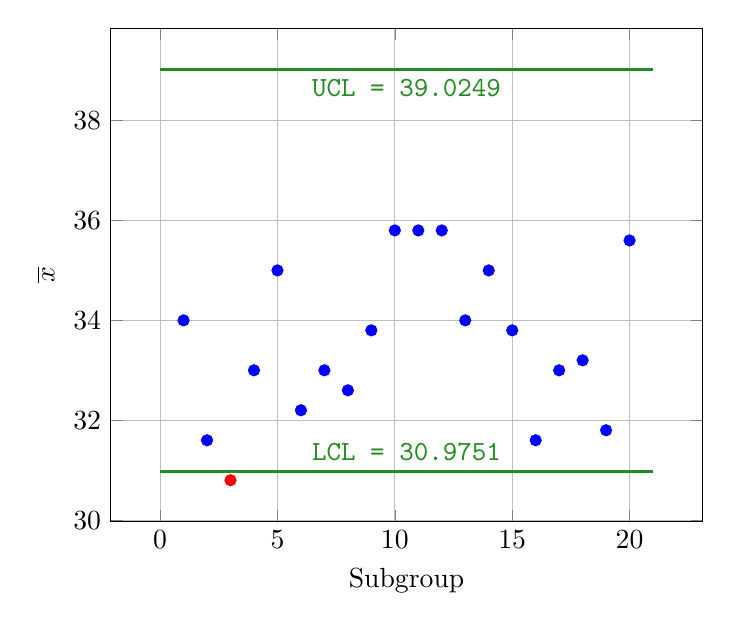
\begin{tikzpicture} 
			\begin{axis}[width = 0.75\textwidth, xlabel = Subgroup, ylabel = $\overline{x}$ , grid = both] 
				\addplot[only marks, color = blue] plot coordinates{(1, 34.0) (2, 31.6) (4, 33.0) (5, 35.0) (6, 32.2) (7, 33.0) (8, 32.6) (9, 33.8) (10, 35.8) (11, 35.8) (12, 35.8) (13, 34.0) (14, 35.0) (15, 33.8) (16, 31.6) (17, 33.0) (18, 33.2) (19, 31.8) (20, 35.6)}; 
				\addplot[only marks, color = red, mark size = 2pt] plot coordinates{(3, 30.8)}; 
				\addplot[mark = none, line width = 1pt, color = ForestGreen, domain = 0:21]{30.9751} node[above, pos = 0.5] {\texttt{LCL = 30.9751}}; 
				\addplot[mark = none, line width = 1pt, color = ForestGreen, domain = 0:21]{39.0249} node[below, pos = 0.5] {\texttt{UCL = 39.0249}}; 
			\end{axis} 
		\end{tikzpicture} 
	\end{figure}

	\item Probability of detection, given $ a,\ \mu,\ \sigma $,
	
	\begin{align}
		P\{\text{detection}\} &= 1 - \Phi\left(3 - \frac{a}{\sigma/\sqrt{n}}\right) \nonumber \\
		%
		&= 29.45\%
	\end{align}

	The mean number of subgroups needed to detect the shift is 3.39\\
	
	\item Given $ Y \sim \chi^2_{n-1} $,
	
	\begin{align}
		\mathbb{E}[\sqrt{Y}] &= \int\limits_{0}^\infty \sqrt{y}\ f(y)\ \mathrm{d}y \\
		%
		&= \int\limits_{0}^\infty \sqrt{y}\ \frac{\lambda^\alpha\ e^{-\lambda y}\ y^{\alpha - 1}}{\Gamma(\alpha)}\ \mathrm{d}y \nonumber \\
		%
		&= \int\limits_{0}^\infty\ \frac{\ e^{-y/2}\ y^{n/2 - 1}}{2^{(n-1)/2}\ \Gamma(\tfrac{n-1}{2})}\ \mathrm{d}y \nonumber \\
		%
		&\text{substitute}\ x = y/2 \nonumber \\
		%
		&= \int\limits_{0}^\infty\ \sqrt{2}\ \frac{\ e^{-x}\ x^{n/2 - 1}}{\ \Gamma(\tfrac{n-1}{2})}\ \mathrm{d}x \nonumber \\
		%
		&= \sqrt{2}\ \frac{\Gamma(\tfrac{n}{2})}{\Gamma(\tfrac{n-1}{2})}
	\end{align}

	\item Assuming process in control, $ \texttt{LCL} = 14.01,\ \texttt{UCL} = 14.57 $\\
	Probability of not violating specifications of $ 14.3 \pm 0.45 $ is $ 96.95\% $\\
	
	\item Excluding subgroups 10 and 15 yields $ \texttt{LCL} = 29.89,\ \texttt{UCL} = 42.15 $\\
	
	\begin{figure}[H] 
		\centering 
		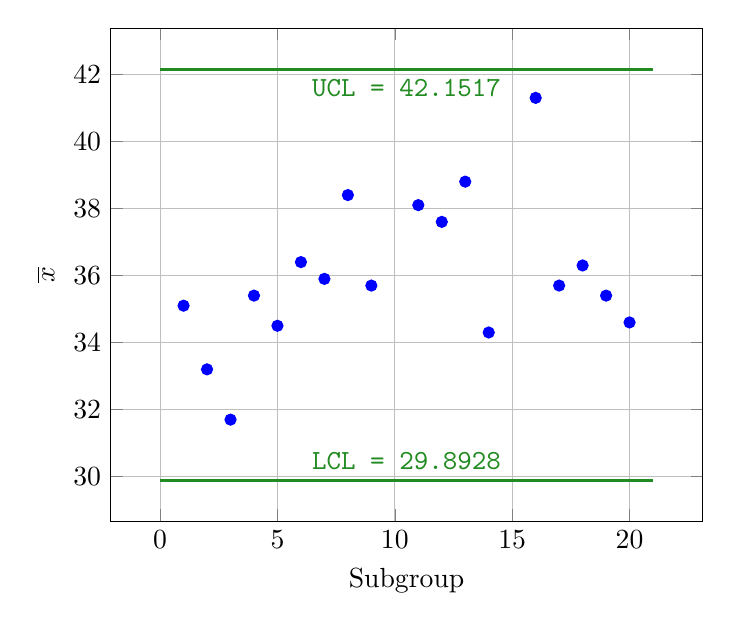
\begin{tikzpicture} 
			\begin{axis}[width = 0.75\textwidth, xlabel = Subgroup, ylabel = $\overline{x}$ , grid = both] 
				\addplot[only marks, color = blue] plot coordinates{(1.0, 35.1) (2.0, 33.2) (3.0, 31.7) (4.0, 35.4) (5.0, 34.5) (6.0, 36.4) (7.0, 35.9) (8.0, 38.4) (9.0, 35.7) (11.0, 38.1) (12.0, 37.6) (13.0, 38.8) (14.0, 34.3) (16.0, 41.3) (17.0, 35.7) (18.0, 36.3) (19.0, 35.4) (20.0, 34.6)}; 
				\addplot[mark = none, line width = 1pt, color = ForestGreen, domain = 0:21]{29.8928} node[above, pos = 0.5] {\texttt{LCL = 29.8928}}; 
				\addplot[mark = none, line width = 1pt, color = ForestGreen, domain = 0:21]{42.1517} node[below, pos = 0.5] {\texttt{UCL = 42.1517}}; 
			\end{axis} 
		\end{tikzpicture} 
	\end{figure}
	
	\begin{figure}[H] 
		\centering 
		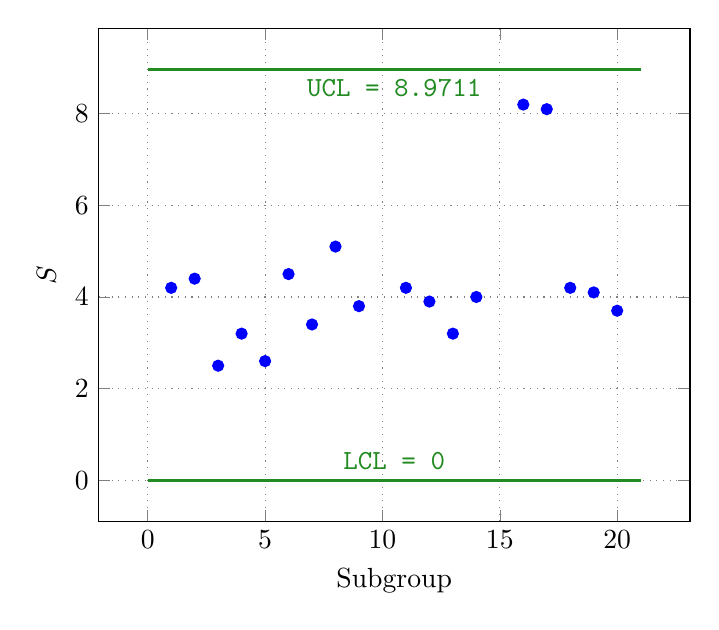
\begin{tikzpicture} 
			\begin{axis}[width = 0.75\textwidth, xlabel = Subgroup, ylabel = $S$ , grid = both, grid style = {gray, dotted}] 
				\addplot[only marks, color = blue] plot coordinates{(1.0, 4.2) (2.0, 4.4) (3.0, 2.5) (4.0, 3.2) (5.0, 2.6) (6.0, 4.5) (7.0, 3.4) (8.0, 5.1) (9.0, 3.8) (11.0, 4.2) (12.0, 3.9) (13.0, 3.2) (14.0, 4.0) (16.0, 8.2) (17.0, 8.1) (18.0, 4.2) (19.0, 4.1) (20.0, 3.7)}; 
				\addplot[mark = none, line width = 1pt, color = ForestGreen, domain = 0:21]{0} node[above, pos = 0.5] {\texttt{LCL = 0}}; 
				\addplot[mark = none, line width = 1pt, color = ForestGreen, domain = 0:21]{8.97} node[below, pos = 0.5] {\texttt{UCL = 8.9711}}; 
			\end{axis} 
		\end{tikzpicture} 
	\end{figure}

	\item The control limits for S-charts are \texttt{LCL} = 0 and \texttt{UCL} = 0.4078 \\
	
	\item Initial control charts for $ \overline{X} $ and $ S $ \\
	\begin{figure}[H] 
		\centering 
		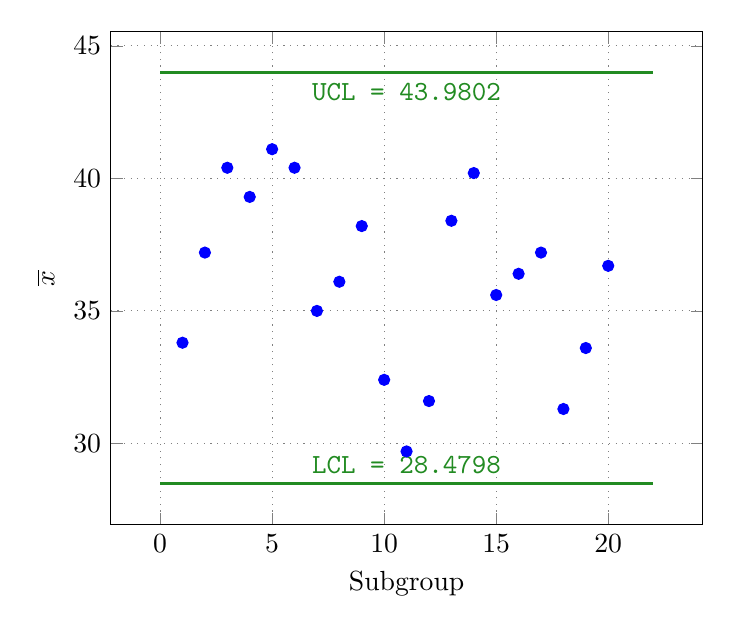
\begin{tikzpicture} 
			\begin{axis}[width = 0.75\textwidth, xlabel = Subgroup, ylabel = $\overline{x}$ , grid = both, grid style = {dotted, gray}] 
				\addplot[only marks, color = blue] plot coordinates{(1.0, 33.8) (2.0, 37.2) (3.0, 40.4) (4.0, 39.3) (5.0, 41.1) (6.0, 40.4) (7.0, 35.0) (8.0, 36.1) (9.0, 38.2) (10.0, 32.4) (11.0, 29.7) (12.0, 31.6) (13.0, 38.4) (14.0, 40.2) (15.0, 35.6) (16.0, 36.4) (17.0, 37.2) (18.0, 31.3) (19.0, 33.6) (20.0, 36.7)}; 
				\addplot[only marks, color = red, mark size = 2pt] plot coordinates{}; 
				\addplot[mark = none, line width = 1pt, color = ForestGreen, domain = 0:22]{28.48} node[above, pos = 0.5] {\texttt{LCL = 28.4798}}; 
				\addplot[mark = none, line width = 1pt, color = ForestGreen, domain = 0:22]{43.98} node[below, pos = 0.5] {\texttt{UCL = 43.9802}}; 
			\end{axis} 
		\end{tikzpicture} 
	\end{figure}
	
	Yes the process was in control throughout.
	
	Fraction of items falling in the range $ 35 \pm 10 $, is 91.25\%\\
	\begin{figure}[H] 
		\centering 
		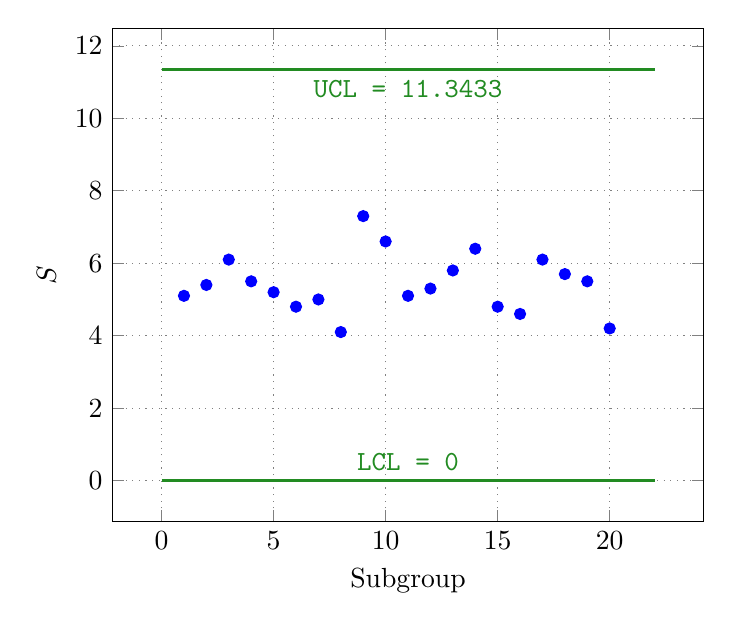
\begin{tikzpicture} 
			\begin{axis}[width = 0.75\textwidth, xlabel = Subgroup, ylabel = $S$ , grid = both, grid style = {dotted, gray}] 
				\addplot[only marks, color = blue] plot coordinates{(1.0, 5.1) (2.0, 5.4) (3.0, 6.1) (4.0, 5.5) (5.0, 5.2) (6.0, 4.8) (7.0, 5.0) (8.0, 4.1) (9.0, 7.3) (10.0, 6.6) (11.0, 5.1) (12.0, 5.3) (13.0, 5.8) (14.0, 6.4) (15.0, 4.8) (16.0, 4.6) (17.0, 6.1) (18.0, 5.7) (19.0, 5.5) (20.0, 4.2)}; 
				\addplot[only marks, color = red, mark size = 2pt] plot coordinates{}; 
				\addplot[mark = none, line width = 1pt, color = ForestGreen, domain = 0:22]{0} node[above, pos = 0.5] {\texttt{LCL = 0}}; 
				\addplot[mark = none, line width = 1pt, color = ForestGreen, domain = 0:22]{11.34} node[below, pos = 0.5] {\texttt{UCL = 11.3433}}; 
			\end{axis} 
		\end{tikzpicture} 
	\end{figure}
	
	\item The control limits for S-charts are \texttt{LCL} = 0 and \texttt{UCL} = 37.77 \\
	The control limits for $ \overline{X} $-charts are \texttt{LCL} = 394.86 and \texttt{UCL} = 449.13 \\
	$ \sigma = \overline{S} / c(n)  = 18.09$\\
	Fraction of products not meeting minimum spec = 11.2\% \\
	
	\item The control limits for S-charts are \texttt{LCL} = 0 and \texttt{UCL} = 50.98 \\
	The control limits for $ \overline{X} $-charts are \texttt{LCL} = 394.36 and \texttt{UCL} = 467.62 \\
	$ \sigma = \overline{S} / c(n)  = 24.42$\\
	Fraction of products meeting spec of $ [430 \pm 30] $ = 78\% \\
	Upon increasing $ \mu \to \mu + 60 $, probability of detection is 97.2\% \\
	
	\item The control limits for S-charts are \texttt{LCL} = 0 and \texttt{UCL} = 0.0224 \\
	The control limits for $ \overline{X} $-charts are \texttt{LCL} = 0.2362 and \texttt{UCL} = 0.2668 \\
	Process is in control, no revision necessary.
	
	\item The control limits for S-charts are \texttt{LCL} = 0.0516 and \texttt{UCL} = 1.7866 \\
	The control limits for $ \overline{X} $-charts are \texttt{LCL} = 17.21 and \texttt{UCL} = 21.59 \\
	$ \sigma = \overline{S} / c(n)  = 1.786$\\
	Fraction of products meeting spec of $ [19 \pm 4] $ = 97.11\% \\
	
	\item Plotting the control charts for fraction of defects in subgroups of size $ n = 100 $\\
	The process is in control\\
	
	\begin{figure}[H] 
		\centering 
		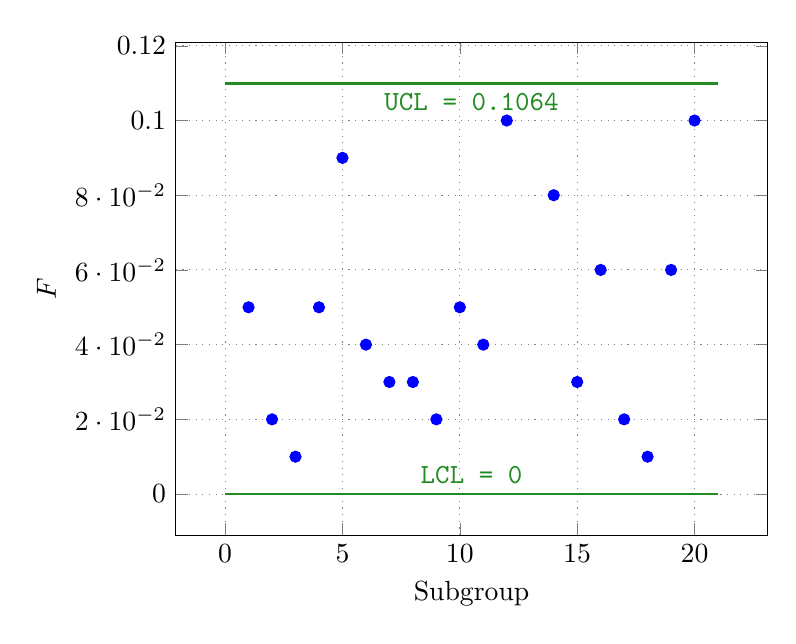
\begin{tikzpicture} 
			\begin{axis}[ylabel near ticks, width = 0.75\textwidth, xlabel = Subgroup, ylabel = $F$ , grid = both, grid style = {dotted, gray}] 
				\addplot[only marks, color = blue] plot coordinates{(1, 0.05) (2, 0.02) (3, 0.01) (4, 0.05) (5, 0.09) (6, 0.04) (7, 0.03) (8, 0.03) (9, 0.02) (10, 0.05) (11, 0.04) (12, 0.1) (14, 0.08) (15, 0.03) (16, 0.06) (17, 0.02) (18, 0.01) (19, 0.06) (20, 0.1)}; 
				\addplot[only marks, color = red, mark size = 2pt] plot coordinates{}; 
				\addplot[mark = none, line width = 1pt, color = ForestGreen, domain = 0:21]{0} node[above, pos = 0.5] {\texttt{LCL = 0}}; 
				\addplot[mark = none, line width = 1pt, color = ForestGreen, domain = 0:21]{0.11} node[below, pos = 0.5] {\texttt{UCL = 0.1064}}; 
			\end{axis} 
		\end{tikzpicture} 
	\end{figure}
	
	\item Plotting the control charts for fraction of defects in subgroups of varying size $ \overline{F} = 0.713 $ \\
	
	\begin{figure}[H] 
		\centering 
		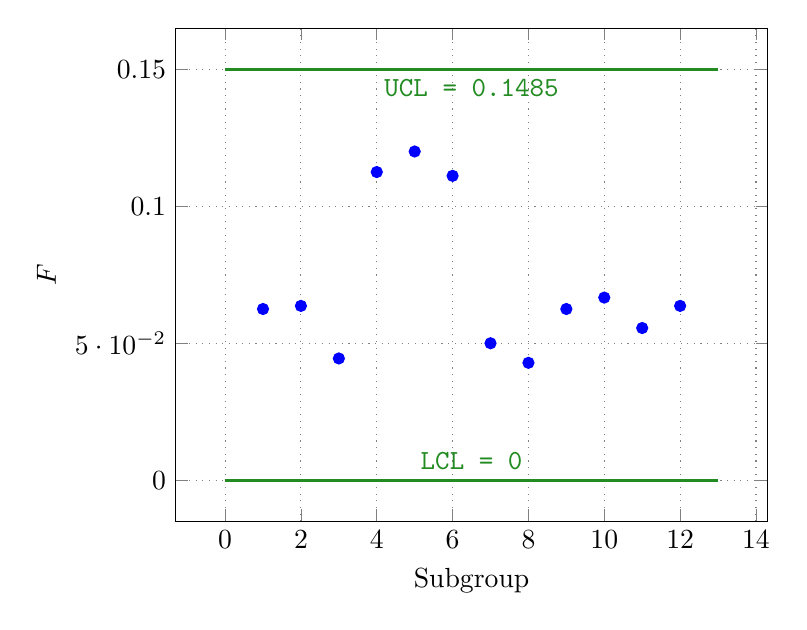
\begin{tikzpicture} 
			\begin{axis}[ylabel near ticks, width = 0.75\textwidth, xlabel = Subgroup, ylabel = $F$ , grid = both, grid style = {dotted, gray}] 
				\addplot[only marks, color = blue] plot coordinates{(1, 0.0625) (2, 0.06363636363636363) (3, 0.044444444444444446) (4, 0.1125) (5, 0.12) (6, 0.1111111111111111) (7, 0.05) (8, 0.04285714285714286) (9, 0.0625) (10, 0.06666666666666667) (11, 0.05555555555555555) (12, 0.06363636363636363)}; 
				\addplot[only marks, color = red, mark size = 2pt] plot coordinates{}; 
				\addplot[mark = none, line width = 1pt, color = ForestGreen, domain = 0:13]{0} node[above, pos = 0.5] {\texttt{LCL = 0}}; 
				\addplot[mark = none, line width = 1pt, color = ForestGreen, domain = 0:13]{0.15} node[below, pos = 0.5] {\texttt{UCL = 0.1485}}; 
			\end{axis} 
		\end{tikzpicture} 
	\end{figure}

	\item $ p = 0.04,\ n = 500 $. Shift in probability such that $ p_1 = 0.08 $\\
	$ P\{\texttt{Binom}(n, p_1) > np\} = $
	The control limits for number defective are \texttt{LCL} = 6.58, \texttt{UCL} = 33.42\\
	Probability of detecting change in parameter $ p $ is 86\% \\
	
	\item Control chart for the number defective (subgroup 1 and 2 trimmed) \\
	
	\begin{figure}[H] 
		\centering 
		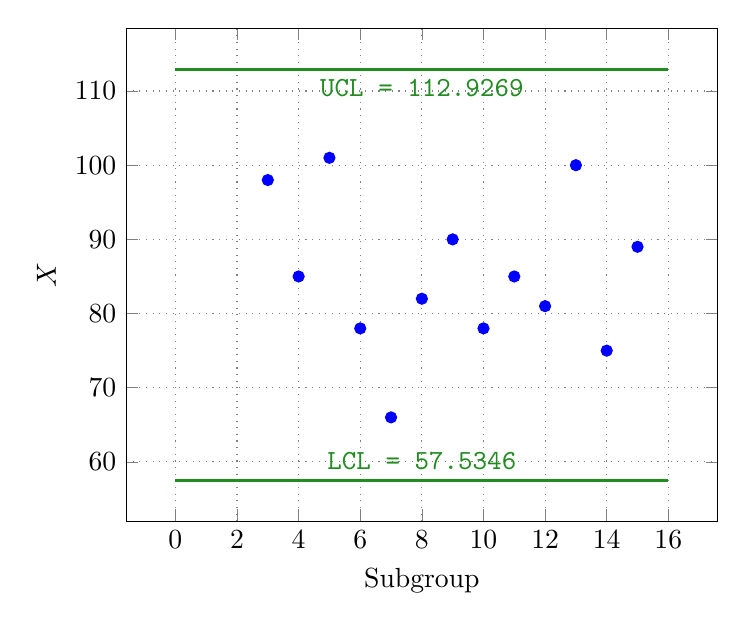
\begin{tikzpicture} 
			\begin{axis}[ylabel near ticks, width = 0.75\textwidth, xlabel = Subgroup, ylabel = $X$ , grid = both, grid style = {dotted, gray}] 
				\addplot[only marks, color = blue] plot coordinates{(3, 98) (4, 85) (5, 101) (6, 78) (7, 66) (8, 82) (9, 90) (10, 78) (11, 85) (12, 81) (13, 100) (14, 75) (15, 89)}; 
				\addplot[only marks, color = red, mark size = 2pt] plot coordinates{}; 
				\addplot[mark = none, line width = 1pt, color = ForestGreen, domain = 0:16]{57.53} node[above, pos = 0.5] {\texttt{LCL = 57.5346}}; 
				\addplot[mark = none, line width = 1pt, color = ForestGreen, domain = 0:16]{112.93} node[below, pos = 0.5] {\texttt{UCL = 112.9269}}; 
			\end{axis} 
		\end{tikzpicture} 
	\end{figure}

	\item Control chart for the number defective (subgroup 14 trimmed)
	
	\begin{figure}[H] 
		\centering 
		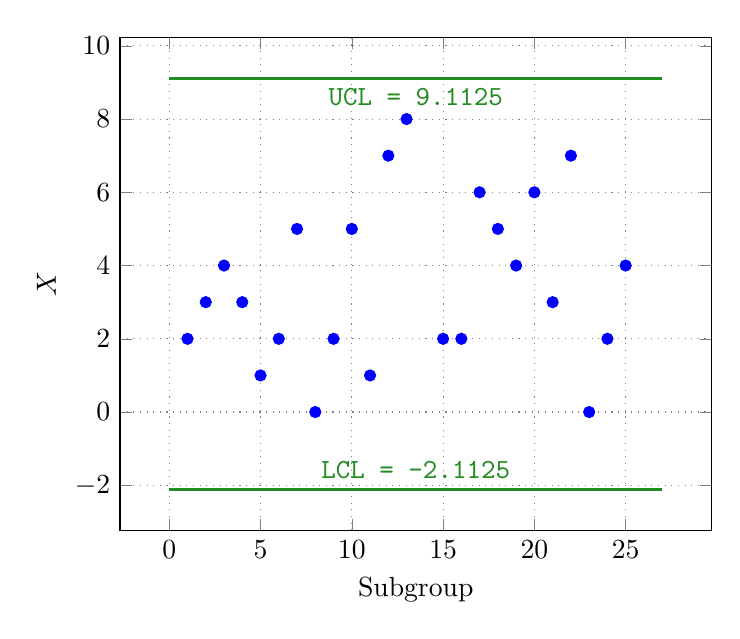
\begin{tikzpicture} 
			\begin{axis}[ylabel near ticks, width = 0.75\textwidth, xlabel = Subgroup, ylabel = $X$ , grid = both, grid style = {dotted, gray}] 
				\addplot[only marks, color = blue] plot coordinates{(1.0, 2.0) (2.0, 3.0) (15.0, 2.0) (3.0, 4.0) (16.0, 2.0) (4.0, 3.0) (17.0, 6.0) (5.0, 1.0) (18.0, 5.0) (6.0, 2.0) (19.0, 4.0) (7.0, 5.0) (20.0, 6.0) (8.0, 0.0) (21.0, 3.0) (9.0, 2.0) (22.0, 7.0) (10.0, 5.0) (23.0, 0.0) (11.0, 1.0) (24.0, 2.0) (12.0, 7.0) (25.0, 4.0) (13.0, 8.0)}; 
				\addplot[only marks, color = red, mark size = 2pt] plot coordinates{}; 
				\addplot[mark = none, line width = 1pt, color = ForestGreen, domain = 0:27]{-2.11} node[above, pos = 0.5] {\texttt{LCL = -2.1125}}; 
				\addplot[mark = none, line width = 1pt, color = ForestGreen, domain = 0:27]{9.11} node[below, pos = 0.5] {\texttt{UCL = 9.1125}}; 
			\end{axis} 
		\end{tikzpicture} 
	\end{figure}

	\item No the process has not been in control throughout. Subgroup 3 and 5 are violators.
	\begin{figure}[H] 
		\centering 
		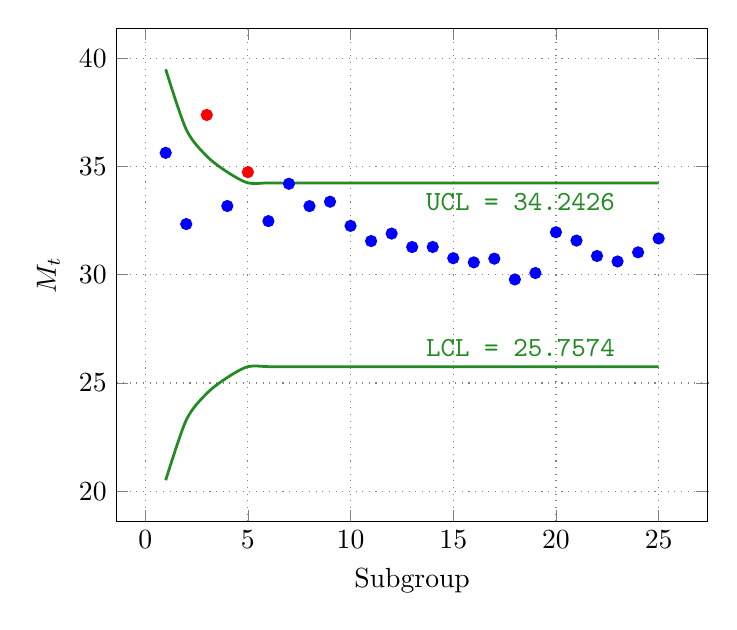
\begin{tikzpicture} 
			\begin{axis}[ylabel near ticks, width = 0.75\textwidth, xlabel = Subgroup, ylabel = $M_t$ , grid = both, grid style = {dotted, gray}] 
				\addplot[only marks, color = blue] plot coordinates{(1, 35.62938) (2, 32.34106) (4, 33.1748) (6, 32.47771) (7, 34.20162) (8, 33.17019) (9, 33.37338) (10, 32.2585) (11, 31.55621) (12, 31.90186) (13, 31.28057) (14, 31.2824) (15, 30.76488) (16, 30.57259) (17, 30.74358) (18, 29.78317) (19, 30.08048) (20, 31.96463) (21, 31.57853) (22, 30.86678) (23, 30.61448) (24, 31.03497) (25, 31.67531)}; 
				\addplot[only marks, color = red, mark size = 2pt] plot coordinates{(3, 37.37978) (5, 34.73976)}; 
				\addplot[mark = none, smooth, line width = 1pt, color = ForestGreen, domain = 0:26] plot coordinates{(1, 20.513167019494862) (2, 23.29179606750063) (3, 24.522774424948338) (4, 25.25658350974743) (5, 25.757359312880716) (6, 25.757359312880716) (7, 25.757359312880716) (8, 25.757359312880716) (9, 25.757359312880716) (10, 25.757359312880716) (11, 25.757359312880716) (12, 25.757359312880716) (13, 25.757359312880716) (14, 25.757359312880716) (15, 25.757359312880716) (16, 25.757359312880716) (17, 25.757359312880716) (18, 25.757359312880716) (19, 25.757359312880716) (20, 25.757359312880716) (21, 25.757359312880716) (22, 25.757359312880716) (23, 25.757359312880716) (24, 25.757359312880716) (25, 25.757359312880716)} node[above, pos = 0.75] {\texttt{LCL = 25.7574}}; 
				\addplot[mark = none, smooth, line width = 1pt, color = ForestGreen, domain = 0:26] plot coordinates{(1, 39.48683298050514) (2, 36.708203932499366) (3, 35.47722557505166) (4, 34.74341649025257) (5, 34.242640687119284) (6, 34.242640687119284) (7, 34.242640687119284) (8, 34.242640687119284) (9, 34.242640687119284) (10, 34.242640687119284) (11, 34.242640687119284) (12, 34.242640687119284) (13, 34.242640687119284) (14, 34.242640687119284) (15, 34.242640687119284) (16, 34.242640687119284) (17, 34.242640687119284) (18, 34.242640687119284) (19, 34.242640687119284) (20, 34.242640687119284) (21, 34.242640687119284) (22, 34.242640687119284) (23, 34.242640687119284) (24, 34.242640687119284) (25, 34.242640687119284)} node[below, pos = 0.75] {\texttt{UCL = 34.2426}}; 
			\end{axis} 
		\end{tikzpicture} 
	\end{figure}

	\item No the process has not been in control throughout. Subgroups 10 onwards are violators.
	\begin{figure}[H] 
		\centering 
		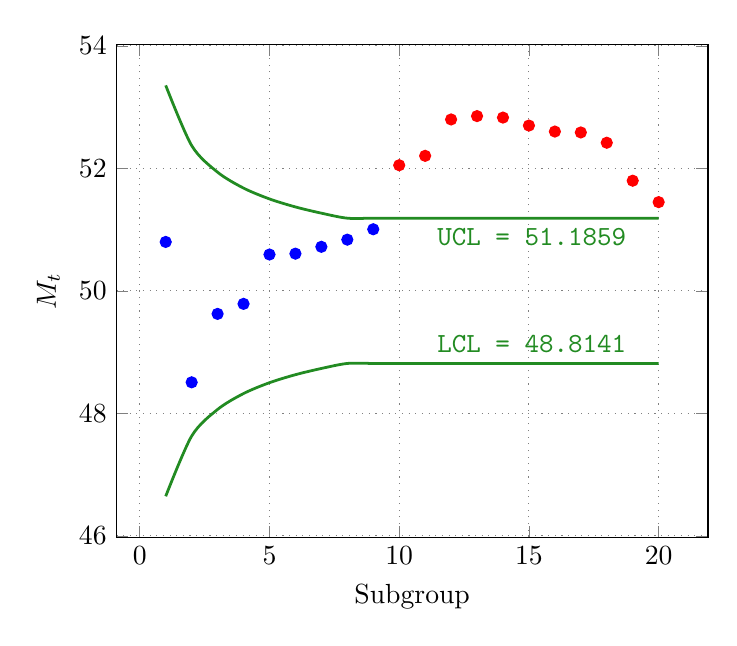
\begin{tikzpicture} 
			\begin{axis}[ylabel near ticks, width = 0.75\textwidth, xlabel = Subgroup, ylabel = $M_t$ , grid = both, grid style = {dotted, gray}] 
				\addplot[only marks, color = blue] plot coordinates{(1, 50.79806) (2, 48.50609) (3, 49.62337) (4, 49.78696) (5, 50.59259) (6, 50.60655) (7, 50.71859) (8, 50.83533) (9, 51.00508)}; 
				\addplot[only marks, color = red, mark size = 2pt] plot coordinates{(10, 52.05022) (11, 52.2036) (12, 52.79759) (13, 52.85237) (14, 52.82834) (15, 52.69814) (16, 52.6002) (17, 52.58531) (18, 52.41748) (19, 51.79759) (20, 51.44783)}; 
				\addplot[mark = none, smooth, line width = 1pt, color = ForestGreen, domain = 0:21] plot coordinates{(1, 46.64589803375031) (2, 47.628291754873715) (3, 48.06350832689629) (4, 48.32294901687516) (5, 48.5) (6, 48.63069360623709) (7, 48.73226861790722) (8, 48.81414587743686) (9, 48.81414587743686) (10, 48.81414587743686) (11, 48.81414587743686) (12, 48.81414587743686) (13, 48.81414587743686) (14, 48.81414587743686) (15, 48.81414587743686) (16, 48.81414587743686) (17, 48.81414587743686) (18, 48.81414587743686) (19, 48.81414587743686) (20, 48.81414587743686)} node[above, pos = 0.75] {\texttt{LCL = 48.8141}}; 
				\addplot[mark = none, smooth, line width = 1pt, color = ForestGreen, domain = 0:21] plot coordinates{(1, 53.35410196624969) (2, 52.371708245126285) (3, 51.93649167310371) (4, 51.67705098312484) (5, 51.5) (6, 51.36930639376291) (7, 51.26773138209278) (8, 51.18585412256314) (9, 51.18585412256314) (10, 51.18585412256314) (11, 51.18585412256314) (12, 51.18585412256314) (13, 51.18585412256314) (14, 51.18585412256314) (15, 51.18585412256314) (16, 51.18585412256314) (17, 51.18585412256314) (18, 51.18585412256314) (19, 51.18585412256314) (20, 51.18585412256314)} node[below, pos = 0.75] {\texttt{UCL = 51.1859}}; 
			\end{axis} 
		\end{tikzpicture} 
	\end{figure}

	\item EWMA on Problem 17 data with $ \alpha = 1/3 $.
	Process out of control at subgroup 3.
	
	\begin{figure}[H] 
		\centering 
		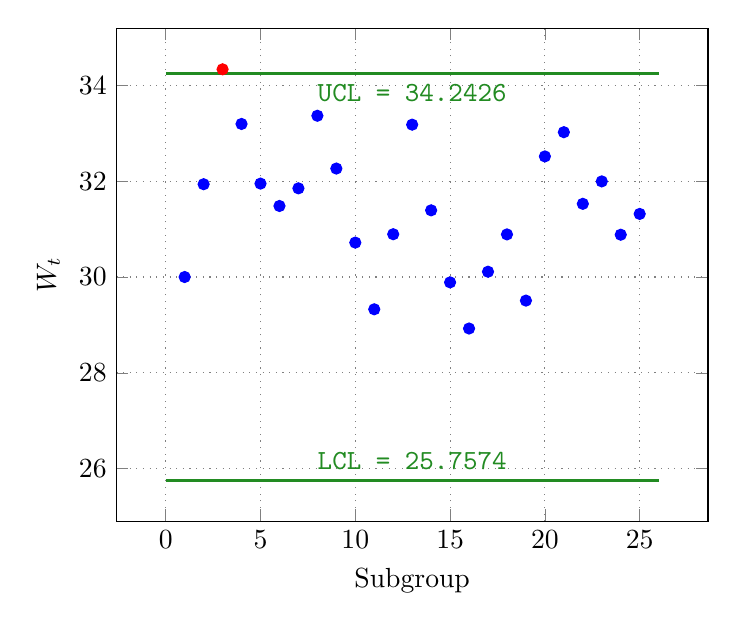
\begin{tikzpicture} 
			\begin{axis}[ylabel near ticks, width = 0.75\textwidth, xlabel = Subgroup, ylabel = $W_t$ , grid = both, grid style = {dotted, gray}] 
				\addplot[only marks, color = blue] plot coordinates{(1, 30.0) (2, 31.936483333333335) (4, 33.19412148148149) (5, 31.949327654320992) (6, 31.482315102880666) (7, 31.850610068587113) (8, 33.365120045724744) (9, 32.26355003048316) (10, 30.718043353655442) (11, 29.326538902436965) (12, 30.89310593495798) (13, 33.17940062330532) (14, 31.39169708220355) (15, 29.888224721469037) (16, 28.925236480979358) (17, 30.110390987319573) (18, 30.88927065821305) (19, 29.507813772142036) (20, 32.51665251476136) (21, 33.02235834317424) (22, 31.52723222878283) (23, 31.995401485855222) (24, 30.882684323903483) (25, 31.31694621593566)}; 
				\addplot[only marks, color = red, mark size = 2pt] plot coordinates{(3, 34.33438222222223)}; 
				\addplot[mark = none, line width = 1pt, color = ForestGreen, domain = 0:26]{25.76} node[above, pos = 0.5] {\texttt{LCL = 25.7574}}; 
				\addplot[mark = none, line width = 1pt, color = ForestGreen, domain = 0:26]{34.24} node[below, pos = 0.5] {\texttt{UCL = 34.2426}}; 
			\end{axis} 
		\end{tikzpicture} 
	\end{figure}

	\item  EWMA on Problem 18 data with $ \alpha = 2/ $.
	Process out of control from subgroup 9 onward.
	\begin{figure}[H] 
		\centering 
		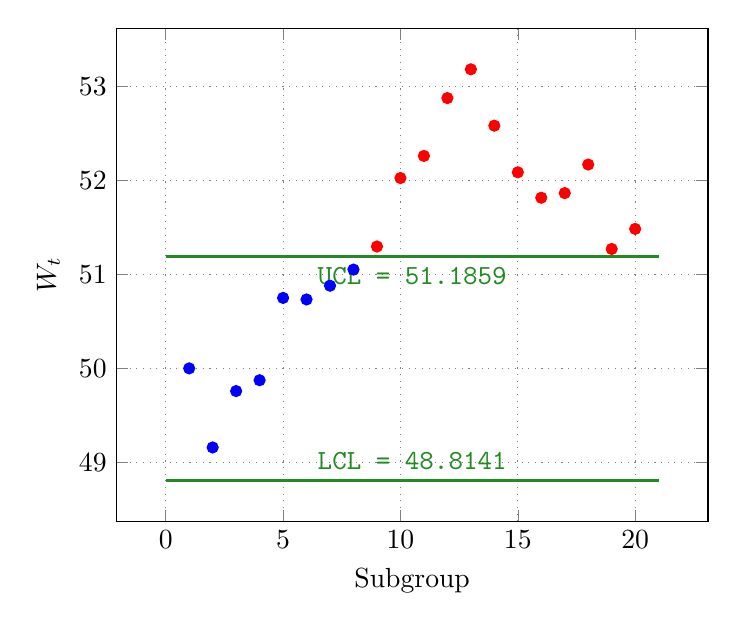
\begin{tikzpicture} 
			\begin{axis}[ylabel near ticks, width = 0.75\textwidth, xlabel = Subgroup, ylabel = $W_t$ , grid = both, grid style = {dotted, gray}] 
				\addplot[only marks, color = blue] plot coordinates{(1, 50.0) (2, 49.15869555555556) (3, 49.75852543209877) (4, 49.87389978052127) (5, 50.74972649596099) (6, 50.733420607969656) (7, 50.8795115839764) (8, 51.05127789864831)}; 
				\addplot[only marks, color = red, mark size = 2pt] plot coordinates{(9, 51.29678725450424) (10, 52.025330086836625) (11, 52.26080562309515) (12, 52.876111040185116) (13, 53.18217080903287) (14, 52.58258840702557) (15, 52.08629764990878) (16, 51.81577817215127) (17, 51.86492746722877) (18, 52.168843585622376) (19, 51.27040723326185) (20, 51.483992292536996)}; 
				\addplot[mark = none, line width = 1pt, color = ForestGreen, domain = 0:21]{48.81} node[above, pos = 0.5] {\texttt{LCL = 48.8141}}; 
				\addplot[mark = none, line width = 1pt, color = ForestGreen, domain = 0:21]{51.19} node[below, pos = 0.5] {\texttt{UCL = 51.1859}}; 
			\end{axis} 
		\end{tikzpicture} 
	\end{figure}

	\item For two kinds of moving average,
	\begin{align}
		\mathrm{Var}(M_t) &= \frac{\sigma^2}{nt} \nonumber \\
		%
		\mathrm{Var}(W_t) &= \frac{\sigma^2}{n}\ \frac{\alpha\ [1 - (1-\alpha)^{2t}]}{(2 - \alpha)} \nonumber 
	\end{align}

	Clearly, $ \mathrm{Var}(M_t) $ is a decreasing function of $ t $, whereas $ \mathrm{Var}(W_t) $ is an increasing function.
	
	Using too many terms in the first $ k-1 $ terms in $ M_t $ would lead to an underestimate of variance which is bad for Type I errors, whereas this is not a problem in the $ W_t $ case.
	
	\item For Problem 17 data, no violation was detected with $ b = 0.25,\ D = 8 $, or with $ b = 0.5,\ D = 4.77 $\\
	
	\begin{figure}[H] 
		\centering 
		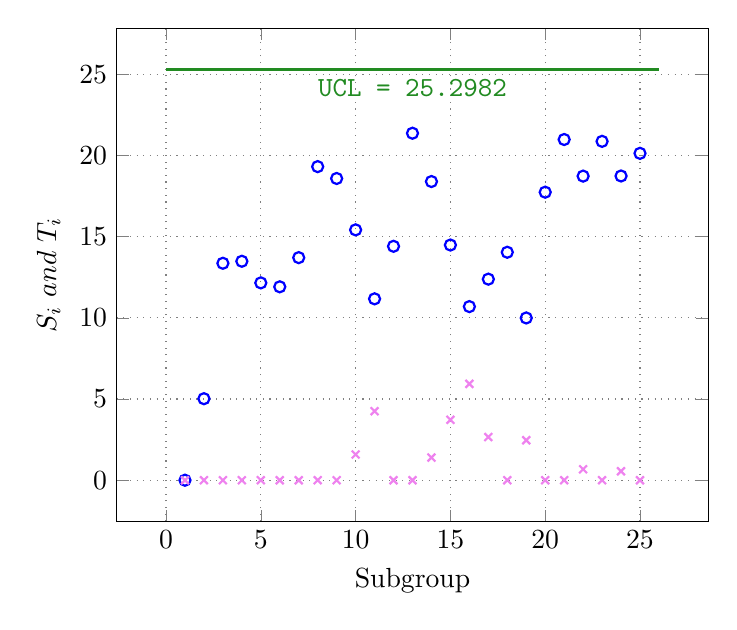
\begin{tikzpicture} 
			\begin{axis}[ylabel near ticks, width = 0.75\textwidth, xlabel = Subgroup, ylabel = $S_i\ \text{and}\ T_i$ , grid = both, grid style = {dotted, gray}] 
				\addplot[thick, only marks, mark = o, color = blue] plot coordinates{(1, 0.0) (2, 5.018880584957904) (3, 13.358491169915812) (4, 13.481521754873716) (5, 12.150692339831622) (6, 11.908412924789529) (7, 13.705043509747437) (8, 19.30861409470534) (9, 18.578454679663245) (10, 15.414915264621152) (11, 11.167875849579058) (12, 14.403546434536965) (13, 21.36496701949487) (14, 18.390687604452772) (15, 14.481398189410678) (16, 10.690088774368583) (17, 12.380219359326487) (18, 14.03667994428439) (19, 9.991010529242297) (20, 17.7347711142002) (21, 20.9779716991581) (22, 18.724382284116004) (23, 20.865552869073905) (24, 18.73223345403181) (25, 20.127134038989716)}; 
				\addplot[thick, only marks, mark = o, color = red, mark size = 2pt] plot coordinates{}; 
				\addplot[thick, only marks, mark = x, color = Violet] plot coordinates{(1, 0.0) (2, 0.0) (3, 0.0) (4, 0.0) (5, 0.0) (6, 0.0) (7, 0.0) (8, 0.0) (9, 0.0) (10, 1.5824005849579037) (11, 4.248301169915808) (12, 0.0) (13, 0.0) (14, 1.3931405849579064) (15, 3.721291169915811) (16, 5.931461754873716) (17, 2.6601923398316223) (18, 0.0) (19, 2.464530584957904) (20, 0.0) (21, 0.0) (22, 0.6724505849579053) (23, 0.0) (24, 0.5521805849579039) (25, 0.0)}; 
				\addplot[thick, only marks, mark = x, color = BrickRed, mark size = 2pt] plot coordinates{}; 
				\addplot[mark = none, line width = 1pt, color = ForestGreen, domain = 0:26]{25.3} node[below, pos = 0.5] {\texttt{UCL = 25.2982}}; 
			\end{axis} 
		\end{tikzpicture} 
	\end{figure}

	\begin{figure}[H] 
		\centering 
		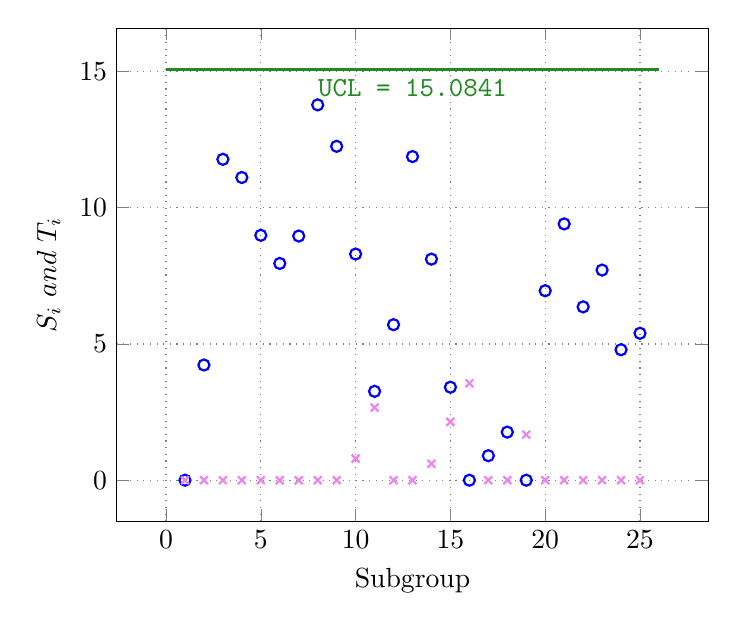
\begin{tikzpicture} 
			\begin{axis}[ylabel near ticks, width = 0.75\textwidth, xlabel = Subgroup, ylabel = $S_i\ \text{and}\ T_i$ , grid = both, grid style = {dotted, gray}] 
				\addplot[thick, only marks, mark = o, color = blue] plot coordinates{(1, 0.0) (2, 4.228311169915808) (3, 11.777352339831621) (4, 11.10981350974743) (5, 8.98841467966324) (6, 7.9555658495790516) (7, 8.961627019494864) (8, 13.774628189410674) (9, 12.253899359326486) (10, 8.299790529242298) (11, 3.2621816991581083) (12, 5.70728286907392) (13, 11.878134038989728) (14, 8.113285208905538) (15, 3.413426378821348) (16, 0.0) (17, 0.899561169915809) (18, 1.7654523398316173) (19, 0.0) (20, 6.953191169915807) (21, 9.405822339831614) (22, 6.361663509747424) (23, 7.712264679663232) (24, 4.788375849579043) (25, 5.392707019494855)}; 
				\addplot[thick, only marks, mark = o, color = red, mark size = 2pt] plot coordinates{}; 
				\addplot[thick, only marks, mark = x, color = Violet] plot coordinates{(1, 0.0) (2, 0.0) (3, 0.0) (4, 0.0) (5, 0.0) (6, 0.0) (7, 0.0) (8, 0.0) (9, 0.0) (10, 0.7918311699158089) (11, 2.6671623398316187) (12, 0.0) (13, 0.0) (14, 0.6025711699158116) (15, 2.1401523398316216) (16, 3.5597535097474324) (17, 0.0) (18, 0.0) (19, 1.673961169915809) (20, 0.0) (21, 0.0) (22, 0.0) (23, 0.0) (24, 0.0) (25, 0.0)}; 
				\addplot[thick, only marks, mark = x, color = BrickRed, mark size = 2pt] plot coordinates{}; 
				\addplot[mark = none, line width = 1pt, color = ForestGreen, domain = 0:26]{15.08} node[below, pos = 0.5] {\texttt{UCL = 15.0841}}; 
			\end{axis} 
		\end{tikzpicture} 
	\end{figure}

	\item For Problem 18 data, positive violation was detected at subgroup 8.
	
	\begin{figure}[H] 
		\centering 
		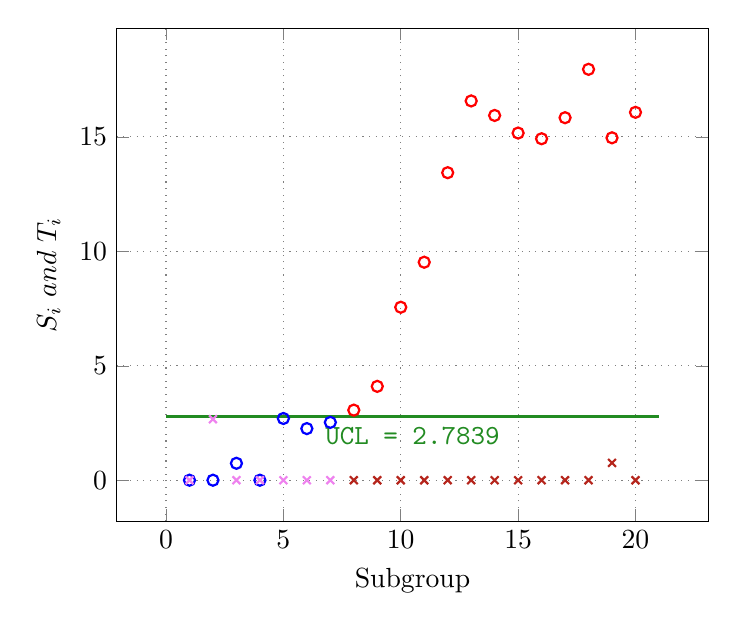
\begin{tikzpicture} 
			\begin{axis}[ylabel near ticks, width = 0.75\textwidth, xlabel = Subgroup, ylabel = $S_i\ \text{and}\ T_i$ , grid = both, grid style = {dotted, gray}] 
				\addplot[thick, only marks, mark = o, color = blue] plot coordinates{(1, 0.0) (2, 0.0) (3, 0.7398960112501083) (4, 0.0) (5, 2.6970860112501054) (6, 2.25540202250021) (7, 2.528198033750316)}; 
				\addplot[thick, only marks, mark = o, color = red, mark size = 2pt] plot coordinates{(8, 3.062624045000419) (9, 4.100660056250524) (10, 7.5578560675006266) (11, 9.52479207875073) (12, 13.436438090000834) (13, 16.57178410125094) (14, 15.93780011250105) (15, 15.169046123751155) (16, 14.919972135001261) (17, 15.838888146251364) (18, 17.953404157501474) (19, 14.961250168751581) (20, 16.07475618000169)}; 
				\addplot[thick, only marks, mark = x, color = Violet] plot coordinates{(1, 0.0) (2, 2.667836011250108) (3, 0.0) (4, 0.0) (5, 0.0) (6, 0.0) (7, 0.0)}; 
				\addplot[thick, only marks, mark = x, color = BrickRed, mark size = 2pt] plot coordinates{(8, 0.0) (9, 0.0) (10, 0.0) (11, 0.0) (12, 0.0) (13, 0.0) (14, 0.0) (15, 0.0) (16, 0.0) (17, 0.0) (18, 0.0) (19, 0.7560860112501029) (20, 0.0)}; 
				\addplot[mark = none, line width = 1pt, color = ForestGreen, domain = 0:21]{2.78} node[below, pos = 0.5] {\texttt{UCL = 2.7839}}; 
			\end{axis} 
		\end{tikzpicture} 
	\end{figure}

\end{enumerate}

